\documentclass[tikz, convert = false]{standalone}

\usepackage[utf8]{inputenx}%  http://ctan.org/pkg/inputenx
% Euler for math | Palatino for rm | Helvetica for ss | Courier for tt
\renewcommand{\rmdefault}{ppl}% rm
\linespread{1.05}% Palatino needs more leading
\usepackage[scaled]{helvet}% ss //  http://ctan.org/pkg/helvet
\usepackage{courier}% tt // http://ctan.org/pkg/courier
\usepackage{eulervm}  %  http://ctan.org/pkg/eulervm
% a better implementation of the euler package (not in gwTeX)
\normalfont%
\usepackage[T1]{fontenc}%  http://ctan.org/pkg/fontenc
\usepackage{textcomp}%  http://ctan.org/pkg/textcomp

\usetikzlibrary{calc}
\usetikzlibrary{intersections}
\usetikzlibrary{shadings}

\begin{document}
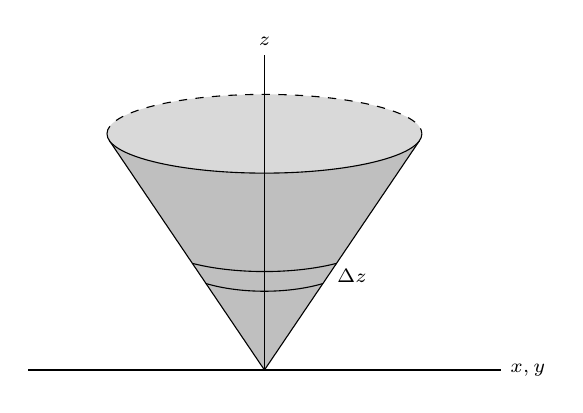
\begin{tikzpicture}
  \pgfmathsetmacro{\a}{asin(0.5/3)}
  \pgfmathsetmacro{\x}{2*cos(\a)}
  \pgfmathsetmacro{\y}{3 - .5*sin(\a)}
  
  \coordinate (h) at (0, 3);
  \coordinate (O) at (0, 0);
   
  \draw[fill = gray!50, name path = tri] (\x, \y) -- (O) -- (-\x, \y);
  \draw[fill = gray!30] (-2, 3) arc[x radius = 2, y radius = .5,
  start angle = 180, end angle = 360];
  \draw[dashed, fill = gray!30] (-2, 3) arc[x radius = 2, y radius = .5,
  start angle = 180, end angle = 0];

  \draw (O) -- +(0, 4) node[font = \scriptsize, above] {$z$};
  \draw (O) -- +(3, 0) node[font = \scriptsize, right] {$x,y$};
  \draw (O) -- +(-3, 0);

  \path[name path = ell1] (0, 1.5) ellipse[x radius = 1.25, y radius = .5];
  \path[name intersections = {of = ell1 and tri}];
  
  \coordinate (P1) at (intersection-3);
  \coordinate (P2) at (intersection-4);

  \begin{scope}
    \clip (P1) rectangle ($(P2) + (0, -1)$);
    \draw (0, 1.5) ellipse[x radius = 1.25, y radius = .5];
  \end{scope}
  
  \path[name path = ell2] (0, 1.75) ellipse[x radius = 1.5, y radius = .5];
  \path[name intersections = {of = ell2 and tri}];

  \coordinate (P3) at (intersection-3);
  \coordinate (P4) at (intersection-4);

  \begin{scope}
    \clip (P3) rectangle ($(P4) + (0, -1)$);
    \draw (0, 1.75) ellipse[x radius = 1.5, y radius = .5];
  \end{scope}

  \node[right, font = \scriptsize] at (.8, 1.2) {$\Delta z$};
\end{tikzpicture} 
\end{document}
%%% Local Variables:
%%% mode: latex
%%% TeX-master: t
%%% End:
